%----------------------------------------
\documentclass[11pt,a4paper, french]{article}
%----------------------------------------
%
\usepackage[french]{babel}
\usepackage{amsmath,amssymb,amsthm}
\usepackage{graphicx}
\usepackage{cancel}
\usepackage{stmaryrd}
\usepackage{hyperref}
\usepackage{xcolor}
\definecolor{blueuppa}{HTML}{67B0E2}
\definecolor{violetuppa}{HTML}{995CA2}
\definecolor{jauneuppa}{HTML}{B3BE11}
\definecolor{vertuppa}{HTML}{5A950E}%8E950E
\hypersetup{
    colorlinks,
    linkcolor={blueuppa!60!black},
    citecolor={blueuppa!30!black},
    urlcolor={blue!80!black}
}
\usepackage{fancyhdr}
\pagestyle{fancy}
\fancyhf{}
\fancyhead[L]{\slshape\nouppercase{\leftmark}}
\fancyhead[R]{\hyperlink{toc}{\thepage}}
%---------------------------------------------------------
\usepackage{tikz-cd}
\newcommand{\cdtriangle}[6]{
\begin{tikzcd}[ampersand replacement=\&] {#1}  \arrow[swap]{rd}{{#4}} \arrow{r}{{#5}}  \& {#2} \arrow{d}{{#6}}\\ \& {#3}  \end{tikzcd}
}
\newcommand{\cdtriangleleft}[6]{
\begin{tikzcd}[ampersand replacement=\&]  {#1} \arrow[swap]{dd}{{#4}} \arrow{dr}{{#5}} \&  \\  \& {#3}\\ {#2} \arrow[swap]{ur}{{#6}} \& \\ \end{tikzcd}
}
\newcommand{\cdsquare}[8]{
\begin{tikzcd}[ampersand replacement=\&] {#1} \arrow{r}{{#5}} \arrow[swap]{d}{{#6}}\& {#2} \arrow{d}{{#7}}\\ {#3} \arrow{r}{{#8}} \& {#4} \end{tikzcd}
}
%----------------------------------------
\usepackage{enumitem}
\setlist[itemize,1]{label=\textbullet}
\setlist[itemize,2]{label=$\triangleright$}
\setlist[itemize,3]{label=$\triangleleft$}
%---------------------------------------------------------
\newcommand{\nparammodel}{n_W}
\newcommand{\ndata}{n_D}
\newcommand{\ndataall}{n_D^*}
\newcommand{\N}{\mathbb N}
\newcommand{\R}{\mathbb R}
\newcommand{\eps}{\varepsilon}
\newcommand{\abs}[1]{\left|#1\right|} 
\newcommand{\norm}[1]{\|#1\|}
\newcommand{\tnorm}[1]{\||#1|\|}
\newcommand{\scp}[2]{\langle#1,#2\rangle}
\newcommand{\sgn}[1]{\operatorname{sgn}(#1)}
\newcommand{\Set}[1]{\left\{#1\right\}} 
\newcommand{\SetDef}[2]{\left\{#1\;\middle|\;#2\right\}} 
\newcommand{\transpose}[1]{{#1}^{\mathsf{T}}} 
\newcommand{\dn}[1]{\frac{\partial{#1}}{\partial n}} 
\renewcommand{\div}{\operatorname{div}}
\newcommand\Rest[2]{{% we make the whole thing an ordinary symbol
  \left.\kern-\nulldelimiterspace % automatically resize the bar with \right
  #1 % the function
  \vphantom{\big|} % pretend it's a little taller at normal size
  \right|_{#2} % this is the delimiter
  }}%
 \newcommand{\vect}[2]{\operatorname{vect}\left\{#1\;\middle|\;#2\right\}} 
 \newcommand{\im}{\operatorname{Im}} 
 \newcommand{\id}{\operatorname{id}} 
%---------------------------------------------------------
\newtheorem{theorem}{Théorème}[section]
\newtheorem{corollary}{Corollaire}[theorem]
\newtheorem{lemma}[theorem]{Lemme}
\newtheorem{algorithm}[theorem]{Algorithme}
\newtheorem{remark}[theorem]{Remarque}
\newtheorem{definition}[theorem]{Définition}
\newtheorem{example}[theorem]{Exemple}
\newtheorem{exercise}[theorem]{Exercice}

%---------------------------------------------------------
\title{M2 MMS : Réseaux de neurones pour la modélisation}
\author{}
\date{\today}
%---------------------------------------------------------

%====================================================
\begin{document}
%====================================================

\maketitle
\tableofcontents
%
%==========================================
\section*{Introduction}\label{sec:}
%==========================================
%
%~~~~~~~~~~~~~~~~~~~~~~~~~~~~~~~~~~~~~~~~~~~~~~~~~~~~~~~~~~~~~~~~~~~~~~~~~~~~~~~~~~~~~~~
\subsection*{Objectifs du cours}\label{subsec:}
%~~~~~~~~~~~~~~~~~~~~~~~~~~~~~~~~~~~~~~~~~~~~~~~~~~~~~~~~~~~~~~~~~~~~~~~~~~~~~~~~~~~~~~~
%
\begin{itemize}
\item Connaître les bases des machines et réseaux de neurones
\item Savoir les utiliser dans le contexte de modèles basées sur les équations différentielles ordinaires (EDO)
\item Savoir utiliser des librairies de l'IA en python.
\end{itemize}
%
Chaque chapitre correspond à 1-3 cours/TP.
%
%~~~~~~~~~~~~~~~~~~~~~~~~~~~~~~~~~~~~~~~~~~~~~~~~~~~~~~~~~~~~~~~~~~~~~~~~~~~~~~~~~~~~~~~
\subsection*{Librairies}\label{subsec:}
%~~~~~~~~~~~~~~~~~~~~~~~~~~~~~~~~~~~~~~~~~~~~~~~~~~~~~~~~~~~~~~~~~~~~~~~~~~~~~~~~~~~~~~~
%
\begin{itemize}
\item \texttt{tensorflow}
\item \texttt{pytorch}
\item \texttt{jax} (avec \texttt{Flax} et \texttt{Optax})
\end{itemize}
%
Prérequis
\begin{itemize}
\item Les base de \texttt{python}
\item \texttt{list}, \texttt{dict}, \texttt{class}
\item \texttt{numpy}
\end{itemize}
%
%==========================================
\section{Machines et réseaux de neurones}\label{sec:}
%==========================================
%
%~~~~~~~~~~~~~~~~~~~~~~~~~~~~~~~~~~~~~~~~~~~~~~~~~~~~~~~~~~~~~~~~~~~~~~~~~~~~~~~~~~~~~~~
\subsection{Machines et exemples classiques}\label{subsec:}
%~~~~~~~~~~~~~~~~~~~~~~~~~~~~~~~~~~~~~~~~~~~~~~~~~~~~~~~~~~~~~~~~~~~~~~~~~~~~~~~~~~~~~~~

%
%--------------------------------------
\begin{definition}\label{definition:}
Soit $m,n,\nparammodel\in\N$. Une \textbf{machine} est une application 
\begin{align*}
\Phi:\R^n\times \R^{\nparammodel}\to \R^m,\qquad (x,\tilde w)\to y = \Phi(x,\tilde w).
\end{align*}
\textbf{L'apprentissage} consiste à déterminer $\tilde w=w_*$ de sorte que l'application $x\mapsto \Phi(x,w_*)$ permet de représenter des données ou un modèle physique.

On appelle $\Phi$ une \textbf{machine vectoriel}, si
\begin{align*}
\Phi(x,\tilde w) = \sum_{i=1}^N c_i \phi_i(x,w).
\end{align*}
Dans ce cas nous avons $\tilde w = (c,w)$ et $X_{\Phi}:=\im\Phi =\vect{\phi_i(x,w)}{1\le i\le N}$.
Les fonction $\phi_i^{w} : x\mapsto \phi_i(x,w)$ peuvent former une base ou non. On les appelle souvent 'features' en anglais. 
Nous avons alors une application ('feature map')
%
\begin{equation}\label{equation:}
\R^{\nparammodel}\to \Set{\R^n\to \R^m}^N\quad w\mapsto (\phi_i^{w})_{1\le i\le N}
\end{equation}
%
%
\end{definition}
%--------------------------------------
%
%
%--------------------------------------
\begin{example}\label{example:}
Voici quelques exemples de machines vectoriels.
\begin{itemize}
\item L'interpolation de Lagrange d'une fonction univariée continue $f:[0;1]\to\R$ avec les points d'interpolation $0 = t_0 < \cdots < t_{i-1}<t_{i} < t_N=1$.
\begin{align*}
I_n f(t) = \sum_{i=0}^N c_i \phi_i(t),\quad \phi_i(t)=\prod_{j=1\atop j\ne i}^{N} \frac{t-t_j}{t_i-t_j}.
\end{align*}
Ici, nous avons "$w=\emptyset$".
\item Même chose, mais avec les points d'interpolation variables, donc "$w=(t_i)$".
\item Espace $P^1([0;1])$. Similaire au deux précédents. On a une base locale, c'est à dire le support de chaque $\phi_i$ est autour de $t_i$.
\item Espace des séries de Fourier tronquées. Similaire aux précédents. Bases globales, le support de chaque $\phi_i$ est tout le domaine.
\end{itemize}
\end{example}
%--------------------------------------
%
%~~~~~~~~~~~~~~~~~~~~~~~~~~~~~~~~~~~~~~~~~~~~~~~~~~~~~~~~~~~~~~~~~~~~~~~~~~~~~~~~~~~~~~~
\subsection{MLP ('multilayer perceptron')}\label{subsec:}
%~~~~~~~~~~~~~~~~~~~~~~~~~~~~~~~~~~~~~~~~~~~~~~~~~~~~~~~~~~~~~~~~~~~~~~~~~~~~~~~~~~~~~~~

%
%--------------------------------------
\begin{definition}\label{definition:}
On appelle \textbf{fonction d'activation} une fonction $\sigma:\R\to\R$.
\begin{enumerate}
\item Sigmoide $\sigma(x) = \frac{1}{1+e^x}$, \quad $\sigma(\R) \subset ]0;1[$.
\item Tanh $\sigma(x) = \tanh(x) = \frac{e^x-e^{-x}}{e^x+e^{-x}}$, \quad $\sigma(\R) \subset ]-1;1[$.
\item ReLU $\operatorname{relu}(x) = x^+ = \max\Set{0,x}$, \quad $\sigma(\R) \subset ]-1;1[$.
\item Swish $\operatorname{swish}(x) = x\sigma(\beta x)$, \quad $\sigma(\R) \subset ]-1;1[$.
\item Id $\sigma(x) = x$, \quad $\sigma(\R) =\R$.
\end{enumerate}
Plein d'autres son possible. Attention : l'image de $\sigma$ est importante.
\end{definition}
%--------------------------------------
%
%
%--------------------------------------
\begin{definition}\label{definition:}
Pour $f:\R\to \R$ on définit $f:\R^n\to\R^n$ (sans distinction de notation !) composante par composante, $\left(f(x)\right)_i = f(x_i), 1\le i\le n$. 

Un \textbf{réseau à une couche ('perceptron')} $(W,b,\sigma), W\in \R^{m\times n}, b\in \R^m$ est l'application 
%
\begin{equation}\label{equation:}
\Phi(x, W,b,\sigma):\R^n\to\R^m,\qquad x \mapsto \sigma(W x + b).
\end{equation}
%
Un \textbf{réseau multi-couches (MLP, 'multi-layer-perceptron')} est la composition de réseau à une couche $\Phi_i=\Phi_i(W_i,b_i,\sigma_i)$, $1\le i\le L$ avec 
%
\begin{equation}\label{equation:}
\Phi(x, \tilde w):\R^n\to \R^m\qquad \Phi(x, \tilde w) = \Phi_L \circ \cdots \circ \Phi_1.
\end{equation}
%
Évidemment nous avons $\tilde w = (W_i,b_i)_{1\le i\le L}$ et
\begin{align*}
W_i\in \R^{n_i\times n_{i-1}},\quad b_i\in \R^{n_i},\quad n_0=n,\quad n_L = m.
\end{align*}
%
\end{definition}
%--------------------------------------
%
%
%--------------------------------------
\begin{remark}\label{remark:}
Un MLP est une machine vectoriel, si $\sigma_L=\id$. Nous avons $N=n_{L-1}$, si $b_L=0$ et  $N=n_{L}$ sinon.
Le fait d'avoir un biais $b_L\ne0$ rajoute la fonction de base $\phi_0=1$, donc, dans ce cas $b_L$ joue aussi le rôle d'un coefficient.
\end{remark}
%--------------------------------------
%
Voici quelques types de couches.
%
\begin{itemize}
\item 'Linear layer avec poids ('weight') $W$ et biais ('bias') $b$'. $x \mapsto W x + b$.
\item 'Activation layer'. $x \mapsto \sigma(x)$.
\item 'Convolutional layer'. Une convolution s'écrit comme une multiplication matrice-vecteur :
\begin{align*}
\textbf{(1D)}\quad y_i = \sum_{k=-m}^m w_k x_{i+k},\quad \textbf{(2D)}\quad y(i,j) = \sum_{k=-m}^m\sum_{l=-m}^m w(k,l) x(i+k, j+l).
\end{align*}

\item 'Residual layer' $\Phi:\R^n\to\R^n$, $\Phi(x) = x +\sigma(W x + b)$
\item 'Attention layer' : $\Phi(x) = {\rm softmax}\left(n^{-1/2} K \transpose{Q}\right)V$ ($K,Q,V\in\R^{n\times n}$)
\begin{align*}
{\rm softmax}_{\beta}: \R^n\to]0;1[^n\quad x\mapsto \left(\frac{e^{\beta x_i}}{\sum_{j=1}^n e^{\beta x_j}}\right)_{1\le i\le n}.
\end{align*}
C'est le gradient de  ${\rm logsumexp}_{\beta}: \R^n\to\R,\quad x\mapsto \beta\log\left(\sum_{j=1}^n e^{\beta x_j}\right)$
\item 'Dropout layer' Il s'agit de réduire le nombre de paramètres de la matrice $W$.
\item 'Implicit layer' Ici $\Phi$ correspond à la solution d'une équation, par exemple une équation différentielle.
\item 'SVM' exemple d'un problème d'optimisation, aussi 'implicit'.
\end{itemize}
%
%
%--------------------------------------
\begin{exercise}\label{exercise:}
\begin{enumerate}
\item Écrire un MLP qui permet de construire l'espace $P^1(h)$ sur un maillage 1D $h=(t_0,\cdots, t_n)$.
\raisebox{-15mm}{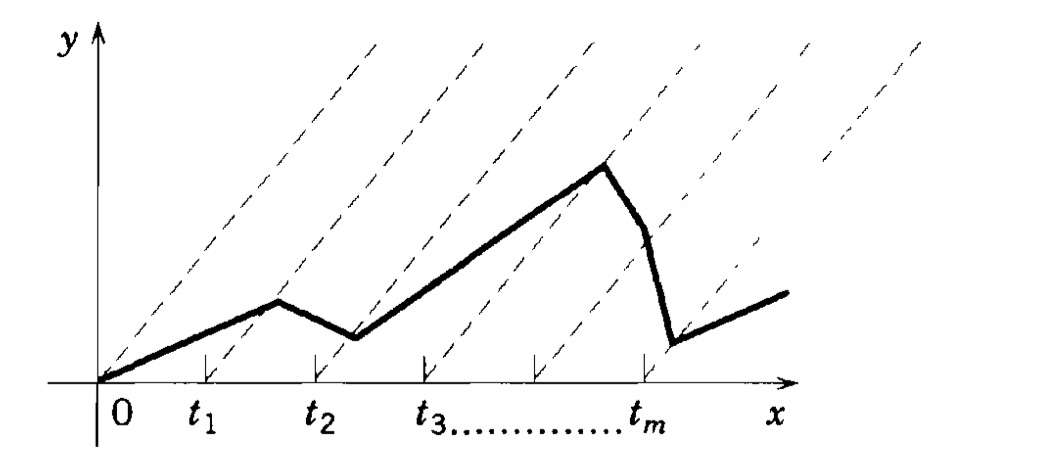
\includegraphics[keepaspectratio = true, width = 0.4\textwidth] {images/P1}}
\item Se servir de la formule pour $k\ge 1$
%
\begin{equation}\label{equation:}
\sum_{j=0}^k b_j t^j + \sum_{i=1}^n a_i (t-t_i)^k_+
\end{equation}
%
pour construire un MLP pour les B-splines.
%
\item Comment construire un MLP pour le $P^1(h)$ sur un maillage en triangles ?
\end{enumerate}
\end{exercise}
%--------------------------------------
%
%==========================================
\section{Pourquoi construire des machines ?}\label{sec:}
%==========================================
%
\begin{itemize}
\item Expliquer les relatons entre $x$ et $y$ : dans le cas unidimensionnel, on interprète de façon géométrique et algébrique $y=a x$ ou $y=bx^2$.
\item Prédire le résultat $y$ associé à un $x$.
\end{itemize}
%
%~~~~~~~~~~~~~~~~~~~~~~~~~~~~~~~~~~~~~~~~~~~~~~~~~~~~~~~~~~~~~~~~~~~~~~~~~~~~~~~~~~~~~~~
\subsection{Différentes classes de problèmes}\label{subsec:}
%~~~~~~~~~~~~~~~~~~~~~~~~~~~~~~~~~~~~~~~~~~~~~~~~~~~~~~~~~~~~~~~~~~~~~~~~~~~~~~~~~~~~~~~
%
\begin{itemize}
%
\item \textbf{Classification (classement)}
\begin{itemize}
\item binaire : il y seulement deux caractéristiques (que l'on peut appeler 0 et 1, $y\in\Set{0,1}$ ou -1 et +1) : chat ou chien, appareil fonctionne ou pas, passager survit à la catastrophe du \textit{Titanic},...
\item classes multiples ('pattern recognition'): reconnaître un chiffre donné $y\in\Set{0,1,\cdots,9}$, différents types de vélos,...
\end{itemize}
%
\item \textbf{Régression} : $y\in\R$ dans le cas scalaire. Étant donné $(x_i,y_i)_{1\le i\le \ndata}$ on cherche $f$ tel que
\begin{align*}
l(f) := \frac{1}{2\ndata}\sum_{i=1}^{\ndata}\left(y_i - f(x_i)\right)^2
\end{align*}
%
soit le plus petit possible. Ce problème dépend de la classe de fonction $f\in\mathcal F$. Si $\mathcal F$ est assez grand nous nous rappelons 
que $l(f_{\rm lag})=0$ pour le polynôme d'interpolation de Lagrange $f_{\rm lag}$, car interpolation signifie $y_i=f(x_i)$.
On se rappelle également que ce processus est instable pour $\ndata\to+\infty$ (et même $\ndata\approx 10$, phénomène de Runge).
%
On s'intéresse plutôt à une classe $\mathcal F$ avec peu de paramètre. Par exemple Gau{\ss} avait pris 
$\mathcal F=\SetDef{x\mapsto a + bx}{a,b\in\R}$, ce qui permet une interprétation des paramètres.
%
\item \textbf{Simplification de modèle} : étant donné un modèle compliqué $\Phi^*$ que l'on ne peut évaluer, on cherche une approximation $\Phi$. Pour l'exemple d'une EDO nonlinéaire \eqref{equation:EDO} 
\begin{align*}
\Phi^* : U\subset\R^n \to C^1(I, \R^n),\quad \Phi^*(u_0) = \mbox{solution de \eqref{equation:EDO} sur l'intervalle $I$}
\end{align*}
Premièrement, $\Phi^*$ ne prend pas des valeurs en un espace de dimension finie. Deuxièmement, on ne connaît pas $\Phi^*(u_0)(t)$ pour un temps $t\in I$. On est obligé de calculer une approximation par une méthode numérique. Et on peut utiliser un réseaux de neuronnes, qui devient alors une méthode numérique. Il y a différentes techniques qui rentre dans cette catégorie
\begin{itemize}
%
\item \textbf{Méthodes de Galerkine} (Séries de Fourier, FEM, ondelettes, méthodes spectrales) où l'on construit des fonctions de base appropriée pour le modèle en question. Ces méthodes dépendent de paramètres. Dans le cas des séries de Fourier il s'agit des indices que l'on utilise et dans le cas de la FEM, il s'agit par exemple du maillage. Depuis longtemps il existe des algorithmes qui cherche à optimiser ces paramètres (méthodes adaptatives) en fonction de la 'solution' $\Phi^*(u_0)$. Il s'agit de l'approximation non-linéaire. 

Une caractéristique des méthode de Galerkine est que les coefficients sont obtenus par la résolution d'un système d'équations nonlinéaires.
Dans les réseaux de neuronnes, même si la machine est vectorielle, on minimise une fonction perte.  
%
\item \textbf{Méthode de réduction de modèle}, POD où on essaie d'extraire l'information essentielle pour construire une base adaptée. Ces méthodes sont souvent combinées avec une méthode de Galerkine.
\end{itemize}
%
\item \textbf{Mélange de régression et de réduction de modèle}. Si nous avons un modèle $\Phi^*$ et des observations (données), on peut facilement combiner les deux si le problème d'apprentissage est une minimisation : il suffit de rajouter une mesure des écarts entre modèle et observations à la fonction à minimiser (la perte). Cela est souvent utilisé comme argument en faveur des réseaux de neuronnes. 
Toutefois, minimiser la somme de deux fonctions $f$ et $g$ dépend d'une pondération que l'on choisit a priori et le résultat peut être très différent des résultats des autres problèmes qui se posent naturellement
\begin{align*}
\left\{
\begin{aligned}
\min\SetDef{f(x)+\alpha g(x)}{x\in\R^n},\\ 
\min\SetDef{f(x)}{x\in\R^n\cap\Set{\norm{g(x)}\le \eps}},\\
\min\SetDef{g(x)}{x\in\R^n\cap\Set{\norm{f(x)}\le \delta}}.
\end{aligned}
\right.
\end{align*}
\end{itemize}
%
%==========================================
\section{Fonction de perte}\label{sec:}
%==========================================
%
%
%--------------------------------------
\begin{definition}\label{definition:}
On appelle \textbf{données} (\textit{data}) un ensemble $\mathcal D=(x_i,y_i)_{1\le i\le \ndata}$, $x_i\in\R^n$, $y\in \R^m$. 
Alors $\mathcal D\subset \R^{\ndataall} \approx \left(\R^n\times \R^m\right)^{\ndata}$. 
Souvent, on partage les données en données d'apprentissage et données de test (et éventuellement données de validation).
\end{definition}
%--------------------------------------
%
%
%--------------------------------------
\begin{definition}\label{definition:Loss}
On appelle \textbf{fonction de perte} (\textit{loss}) une fonction $\widetilde{L}:\R^{\nparammodel}\times\R^{\ndataall}\to \R$ dont la minimisation est l'\textbf{apprentissage} (\textit{learning}). On suppose avoir $L:\R^m\times \R^m\to \R$ telle que
%
\begin{equation}\label{equation:LossForData}
\widetilde{L}(w,\mathcal D) = \frac{1}{\ndata}\sum_{i=1}^{\ndata} L(\Phi(x_i,w),y_i).
\end{equation}
%
Le problème d'apprentissage est alors la minimisation de $\widehat{L}:\R^{\nparammodel}\to\R$
%
\begin{equation}\label{equation:Loss}
\min\SetDef{\widehat{L}(w)}{w\in \R^p},\quad \widehat{L}(w) = \widetilde{L}(w,\mathcal D).
\end{equation}
%
\end{definition}
%--------------------------------------
%
%
%--------------------------------------
\begin{remark}\label{remark:}
On peut avoir une régularisation $\widehat{L}(w) = \widetilde{L}(w,\mathcal D) + \frac{\alpha}{2}\norm{w-w_0}^2$ avec $w_0$ des valeurs données des paramètres du modèle, ou, encore plus complexe, des contraintes sur les paramètres du modèle.
\end{remark}
%--------------------------------------
%
%
%--------------------------------------
\begin{example}\label{example:}
\begin{itemize}
\item (moindre carrés, $l^2$) $L(z,y)= \frac12\norm{y-z}^2$.
\item ($l^1$) $L(z,y)= \norm{y-z}_{l^1(\R^m)}$.
\end{itemize}
\end{example}
%--------------------------------------
%
%~~~~~~~~~~~~~~~~~~~~~~~~~~~~~~~~~~~~~~~~~~~~~~~~~~~~~~~~~~~~~~~~~~~~~~~~~~~~~~~~~~~~~~~
\subsection{Classification binaire}\label{subsec:}
%~~~~~~~~~~~~~~~~~~~~~~~~~~~~~~~~~~~~~~~~~~~~~~~~~~~~~~~~~~~~~~~~~~~~~~~~~~~~~~~~~~~~~~~
%
On utilise souvent la 'binary cross entropy' (si la dernière couche finit avec une sigmoïde)
%
\begin{equation}\label{equation:}
y_i \in \Set{-1,+1},\quad l(x) := -\frac{1}{\ndata}\sum_{i=1}^{\ndata} y_i\log(z_i)+(1-y_i)\log(1-z_i);\quad z_i = \Phi(x_i,w)
\end{equation}
%
%
%~~~~~~~~~~~~~~~~~~~~~~~~~~~~~~~~~~~~~~~~~~~~~~~~~~~~~~~~~~~~~~~~~~~~~~~~~~~~~~~~~~~~~~~
\subsection{Classification}\label{subsec:}
%~~~~~~~~~~~~~~~~~~~~~~~~~~~~~~~~~~~~~~~~~~~~~~~~~~~~~~~~~~~~~~~~~~~~~~~~~~~~~~~~~~~~~~~
%
Avec $n_C$ classes, $y_{ij}\ge0 $, $\sum_{j=1}^{n_C}y_{ij}=1$ pour tout $i$. 
%
\begin{equation}\label{equation:}
y_i \in \llbracket 1,\cdots, n_c\rrbracket \quad l(x) := -\frac{1}{\ndata}\sum_{i=1}^{\ndata}\sum_{j=1}^{n_C} y_{ij}\log(z_{ij});\quad z_{ij} = \Phi(x_i,w).
\end{equation}
%
On interprète les $z_{ij}$ comme la probabilité que 
%
%~~~~~~~~~~~~~~~~~~~~~~~~~~~~~~~~~~~~~~~~~~~~~~~~~~~~~~~~~~~~~~~~~~~~~~~~~~~~~~~~~~~~~~~
\subsection{Moindre carré}\label{subsec:}
%~~~~~~~~~~~~~~~~~~~~~~~~~~~~~~~~~~~~~~~~~~~~~~~~~~~~~~~~~~~~~~~~~~~~~~~~~~~~~~~~~~~~~~~
%
%
\begin{equation}\label{equation:}
l(x)= \frac12\sum_{i=1}^m \abs{y_i-\Phi(x_i,w)}^2.
\end{equation}
%
%
%~~~~~~~~~~~~~~~~~~~~~~~~~~~~~~~~~~~~~~~~~~~~~~~~~~~~~~~~~~~~~~~~~~~~~~~~~~~~~~~~~~~~~~~
\subsection{Remarques}\label{subsec:}
%~~~~~~~~~~~~~~~~~~~~~~~~~~~~~~~~~~~~~~~~~~~~~~~~~~~~~~~~~~~~~~~~~~~~~~~~~~~~~~~~~~~~~~~
%
Il y a une certaine ambiguïté dans nos définition de couches et de fonction de perte : on peut toujours intégrer les dernières couches dans la fonction de parte.
%
%
%--------------------------------------
\begin{theorem}\label{theorem:}
Si la machine contient une couche de la forme $x\to \sigma(Wx+b)$, on peut modifier la fonction de perte telle que la machine est vectorielle.
\end{theorem}
%--------------------------------------
%
%
%--------------------------------------
\begin{proof}
On écrite $x\mapsto\Phi(x,W,b) = \sigma(Wx+b)$ comme $\Phi_2 \circ \Phi_1$ avec $x\mapsto \Phi_1(x,W) = Wx$ et $y\mapsto\Phi_2(y,b) = \sigma(y+b)$. On a alors
\begin{align*}
L(\Phi(x,W,b), y) = L_2(\Phi_1(x,W),y),\quad L_2 (x,y) := L(\Phi_2(x),y).
\end{align*}
\end{proof}
%--------------------------------------
%
%
%--------------------------------------
\begin{example}\label{example:}
Pour les problème de classification on utilise généralement la fonction logistique.
\end{example}
%--------------------------------------
%
%
%==========================================
\section{Apprentissage}\label{sec:}
%==========================================
%
%
%--------------------------------------
\begin{definition}\label{definition:}
Un problème d'apprentissage de machine 'machine learning' consiste en trois ingrédients
\begin{itemize}
\item Une machine $\Phi(x,w)$
\item Une fonction de perte (ce qui implique généralement les données et pratiquement leur traitement)
\item Un algorithme d'optimisation (y compris critère d'arrêt).
\end{itemize}
\end{definition}
%--------------------------------------
%
Ces ingrédients étant fixés, l'apprentissage consiste alors à minimiser la fonction, voir \eqref{equation:LossForData} at \eqref{equation:Loss}
%
\begin{equation}\label{equation:Lossf}
f: \R^{n_W}\to \R,\quad w\mapsto f(w) := \widehat{L}(w) \left( = \frac{1}{\ndata}\sum_{i=1}^{\ndata} L(\Phi(x_i,w),y_i) \right).
\end{equation}
%
Cette fonction est différentiable dans beaucoup de cas (sauf ReLU), mais d'autres propriétés comme la convexité ne sont souvent pas présente.
%
%~~~~~~~~~~~~~~~~~~~~~~~~~~~~~~~~~~~~~~~~~~~~~~~~~~~~~~~~~~~~~~~~~~~~~~~~~~~~~~~~~~~~~~~
\subsection{Méthode de gradient}\label{subsec:}
%~~~~~~~~~~~~~~~~~~~~~~~~~~~~~~~~~~~~~~~~~~~~~~~~~~~~~~~~~~~~~~~~~~~~~~~~~~~~~~~~~~~~~~~
%
En général, les méthodes numériques utilisées dans l'apprentissage sont de variation de la méthode du gradient (ou de la descente).
Partant d'un ensemble de paramètres $w_0\in \R^{n_W}$, on définit
%
\begin{equation}\label{equation:IterationGradient}
w_{k+1} := w_k + t_k \nabla f(w_k),\quad \mbox{$t_k$ est le pas ou 'learning rate'}
\end{equation}
%
Une itération est souvent appelé 'epoch'. L'ingrédient essentiel dans \eqref{equation:IterationGradient} et la gradient.
%
%--------------------------------------
\begin{definition}\label{definition:grad}
Soit $(X,\scp{\cdot}{\cdot})$ un espace de Hilbert et  $f\in C^1(X,\R)$. Alors
%
\begin{equation}\label{equation:}
\scp{\nabla f(x)}{p} := \lim_{s\searrow0}\frac{f(x+sp)-f(x)}{s}.
\end{equation}
%
On note que $\nabla f(x) = \transpose{Df(x)}$ (voir définition~\ref{definition:deriv}).
\end{definition}
%--------------------------------------
%
On voit qu'une difficulté majeure est le calcul de gradient.
%
%~~~~~~~~~~~~~~~~~~~~~~~~~~~~~~~~~~~~~~~~~~~~~~~~~~~~~~~~~~~~~~~~~~~~~~~~~~~~~~~~~~~~~~~
\subsection{Calcul différentiel}\label{subsec:}
%~~~~~~~~~~~~~~~~~~~~~~~~~~~~~~~~~~~~~~~~~~~~~~~~~~~~~~~~~~~~~~~~~~~~~~~~~~~~~~~~~~~~~~~
%
%
On rappelle les notations du calcul différentiel. 
%
%--------------------------------------
\begin{definition}\label{definition:deriv}
$F:\R^n\to\R^m$ est différentiable en $x$ s'il existe $A\in\R^{m\times n}$ tel que 
\begin{align*}
\lim_{h\to 0\atop h\ne0}\frac{\norm{R(x,h)}}{\norm{h}} = 0\quad \left(R(x,h) := F(x+h)-F(x) - Ah\right),\quad DF(x) := A.
\end{align*}
Pour des fonctions de plusieurs variables, par exemple $F(x,z)$ on écrit 
$DF_x(x,z)$ et $DF_z(x,z)$ pour les dérivées  "partielles".
\end{definition}
%--------------------------------------
%
On rappelle également
%
%--------------------------------------
\begin{theorem}\label{theorem:}
Soit $m,n,p\in\N$, $U\subset\R^n$, $V\subset \R^m$, $F\in C^1(U,\R^m)$, $G\in C^1(V,\R^p)$ et $F(U)\subset V$. Alors $h := g\circ f\in C^1(U,\R^p)$ et 
pour $x\in U$ et $y:=f(x)\in V$
%
\begin{equation}\label{eq:calcdiff_deriveecompo}
Dh(x) = Dg(y) Df(x),\quad\cdtriangle{U}{V}{\R^m}{h}{f}{g},\quad\cdtriangle{\R^n}{\R^n}{\R^m}{Dh(x)}{Df(x)}{Dg(y)}.
\end{equation}
%
\end{theorem}
%--------------------------------------
%

Par les théorèmes du calcul différentiel nous avons.
%
%--------------------------------------
\begin{theorem}\label{theorem:}
Si $L$ et $\Phi$ sont continûment différentiables, alors   $\widetilde{L}\in C^1(\R^{\nparammodel})$, le gradient de $\widetilde{L}$ s'écrit
%
\begin{equation}\label{equation:}
\nabla  \widetilde{L}(w) = \frac{1}{\ndata}\sum_{i=1}^{\ndata} \transpose{\Phi'_w(x_i,w)}\nabla_z L(\Phi(x_i,w),y_i)
\end{equation}
%
\end{theorem}
%--------------------------------------
%
%
%~~~~~~~~~~~~~~~~~~~~~~~~~~~~~~~~~~~~~~~~~~~~~~~~~~~~~~~~~~~~~~~~~~~~~~~~~~~~~~~~~~~~~~~
\subsection{Différentiation automatique}\label{subsec:}
%~~~~~~~~~~~~~~~~~~~~~~~~~~~~~~~~~~~~~~~~~~~~~~~~~~~~~~~~~~~~~~~~~~~~~~~~~~~~~~~~~~~~~~~
%
%
%~~~~~~~~~~~~~~~~~~~~~~~~~~~~~~~~~~~~~~~~~~~~~~~~~~~~~~~~~~~~~~~~~~~~~~~~~~~~~~~~~~~~~~~
\subsection{Apprentissage par étape}\label{subsec:}
%~~~~~~~~~~~~~~~~~~~~~~~~~~~~~~~~~~~~~~~~~~~~~~~~~~~~~~~~~~~~~~~~~~~~~~~~~~~~~~~~~~~~~~~
%
%
%
%==========================================
\section{EDO et méthode de collocation}\label{sec:}
%==========================================
%
On considère $U\subset \R^n$ ouvert, $u_0\in U$ et une fonction $f\in C^1(U,\R^n)$. L'équation différentielle ordinaire (EDO) d'ordre un autonome
%
\begin{equation}\label{equation:EDO}
\left\{
\begin{aligned}
\frac{du}{dt} = f(u)\\
u(0) = u_0.
\end{aligned}
\right.
\end{equation}
%
On rappelle le théorème de Cauchy-Lipschitz. S'il existe $r>0$ et $L>0$ tel que
%
\begin{equation}\label{equation:CondLip}
\norm{f(u)-f(v)}\le L\norm{u-v}\quad \forall u,v\in U\cap B_r(u_0),
\end{equation}
%
alors il existe $T>0$ et une solution unique de \eqref{equation:EDO} sur $[0,T]$. $f\in C^1(U,\R^n)$ est suffisant pour \eqref{equation:CondLip}.
%
%
%--------------------------------------
\begin{remark}\label{remark:}
\begin{enumerate}
\item Il existe un temps maximal $T\in\R\cup\Set{+\infty}$ d'existence de solution. Si $T<+\infty$, nous avons $\lim\limits_{t\nearrow T}\abs{u(t)}=+\infty$.
\item L'équation non-autonome
\begin{align*}
\frac{du}{dt} = f(t,u)
\end{align*}
 s'écrite comme \eqref{equation:EDO} avec $\widetilde{u} = (u, v)$, $\widetilde{f}(\widetilde{u}) = (f(v,u),1)$ et $\widetilde{u_0}=(u_0,0)$, la variable $v$ est le temps.
\end{enumerate}
\end{remark}
%--------------------------------------
%
%~~~~~~~~~~~~~~~~~~~~~~~~~~~~~~~~~~~~~~~~~~~~~~~~~~~~~~~~~~~~~~~~~~~~~~~~~~~~~~~~~~~~~~~
\subsection{Méthode de collocation et méthode de Galerkin}\label{subsec:}
%~~~~~~~~~~~~~~~~~~~~~~~~~~~~~~~~~~~~~~~~~~~~~~~~~~~~~~~~~~~~~~~~~~~~~~~~~~~~~~~~~~~~~~~
%
%------------------------------------
\subsubsection{Méthode de collocation}
%------------------------------------

Une méthode de collocation sur un intervalle $I=[0;T]$ consiste à choisir un espace $X_N\subset C^1(I,\R^n)$ de dimension $N+1$ et des points (maillage)
%
\begin{equation}\label{equation:Mesh}
\tau = \left( 0 = t_0 < t_1 < \cdots < t_N = T\right).
\end{equation}
%
On impose les équations à une fonction $u_N\in X_N$
%
\begin{equation}\label{equation:Collocation}
u(0) = u_0,\quad \frac{du}{dt}(t_i) = f(u(t_i))\quad 1\le i\le N.
\end{equation}
%
Soit $(\phi_j)_{0\le j\le N}$ une base de $X_N$. \eqref{equation:Collocation} est alors converti en un système algébrique pour les coefficient $c\in\R^{N+1}$
\begin{align*}
u(t) = \sum_{j=0}^N c_j \phi_j(t),\quad \sum_{j=0}^N c_j \phi_j(0) = u_0,\quad \sum_{j=0}^N c_j\frac{d\phi_j}{dt}(t_i) = f(\sum_{j=0}^N c_j \phi_j(t)).
\end{align*}
%
%
%--------------------------------------
\begin{remark}\label{remark:}
Pour une équation linéaire $f(u)=A u + b$ on obtient un système linéaire à résoudre
%
\begin{equation}\label{equation:}
K c = \gamma,\quad K_{ij} = \frac{d\phi_j}{dt}(t_i) - A\phi_j(t_i),\quad \gamma_i = b 
\end{equation}
%
\end{remark}
%--------------------------------------
%
%
%--------------------------------------
\begin{example}\label{example:}
Pour $X_N = B^1(I)$, l'espace des spline quadratique de classe $C^1$ sur le \textbf{même} maillage $(t_i)_{0\le i\le N}$ on obtient un schéma de type Crank-Nicoloson. Plus généralement, les méthodes de collocation font partie des méthode de Runge-Kutta implicites.
\end{example}
%--------------------------------------
%
%
%------------------------------------
\subsubsection{Méthode de Galerkin}
%------------------------------------
%
Une méthode de Galerkin consiste à choisir deux espaces $X_N$ et $Y_N$ associé à $\tau$ et l'approximation est définie par
%
\begin{equation}\label{equation:}
u\in u_0+X_N :\;\int_0^T \frac{du}{dt} v =  \int_0^T f(u) v\quad \forall v\in Y_n.
\end{equation}
%
%
%~~~~~~~~~~~~~~~~~~~~~~~~~~~~~~~~~~~~~~~~~~~~~~~~~~~~~~~~~~~~~~~~~~~~~~~~~~~~~~~~~~~~~~~
\subsection{Fonction loss}\label{subsec:}
%~~~~~~~~~~~~~~~~~~~~~~~~~~~~~~~~~~~~~~~~~~~~~~~~~~~~~~~~~~~~~~~~~~~~~~~~~~~~~~~~~~~~~~~
%
Une première idée  (PINN) est d'utiliser un espace $\tilde X=X_{\Phi}$ généré par une machine vectorielles $\Phi$ est d'utiliser la fonction perte
\begin{align*}
\frac12\norm{\tilde u(0)-u_0}^2 + \sum_{i=0}^N \frac12\norm{\frac{d\tilde u}{dt}(t_i) - f(\tilde u(t_i)}^2
\end{align*}
Il est alors facile de rajouter un term avec des données $\mathcal D=(\tilde t_k, \tilde w_k)$ (mesures expermientales)
\begin{align*}
l_{\rm PINN}(\tilde u) = \frac12\norm{\tilde u(0)-u_0}^2 + \sum_{i=0}^N \frac12\norm{\frac{d\tilde u}{dt}(t_i) - f(\tilde u(t_i)}^2 + \sum_{k=1}^d \frac12\norm{\tilde u(\tilde t_k) - \tilde w_k}^2
\end{align*}
%
%
%--------------------------------------
\begin{remark}\label{remark:}
Dans le cas sans données ($d=0$), si le MLP produit $B^1(I)$, la machine produit la solution de Crank-Nicolson. Une difficulté est 
le conditionnement du problème.
\end{remark}
%--------------------------------------
%
%
%==========================================
\section{Réseaux pour les EDO}\label{sec:}
%==========================================
%
\begin{enumerate}
\item Pour l'exemple de l'EDO d'ordre deux scalaire
\begin{enumerate}
\item Que se passe-t-il si l'on a plus de fonctions de base que de points de collocations ?
\item Étudier la convergence et l'erreur en fonction du nombre de point de collocation (et du nombre de fonctions de base).
\item Changer les conditions de limites : on remplace $u(T)=0$ par $u'(0)=\alpha$.
\item Que se passe-t-il si l'on varie le nombre de couches ?
\item Que se passe-t-il si l'on change la fonction d'activation ?
\item Que se passe-t-il si l'on change la perte : par exemple pondération différente, $l_1$ ?
\item Essayer d'implémenter les conditions de bord comme contraintes.
\item Plotter les fonctions de base
\end{enumerate}
\end{enumerate}
%
%==========================================
\section{EDO avec paramètres}\label{sec:}
%==========================================
%
Dans la pratique, les modèles mathématiques contiennent des paramètres (physique ou non). Soit $n_p\in\N$ et $p=(p_0,p_1)\in \R^{n_p}$ et
%
\begin{equation}\label{equation:EDOParam}
\left\{
\begin{aligned}
\frac{du}{dt} = f(u,p_1)\\
u(0) = u_0(p_0).
\end{aligned}
\right.
\end{equation}
%
Nous avons alors une application
%
\begin{equation}\label{equation:SolutionOp}
S:\R^{n_p}\to C^1(I,\R^n)\qquad p \to u(p).
\end{equation}
%
%
Des questions typiques sont
\begin{itemize}
\item Déterminer des paramètres à partir de mesures.
\item Plus modestement : déterminer la sensibilité des solution par rapport aux paramètre.
\item Plus ambitieux : déterminer les mesures les plus importantes.
\item Dans un autre registre : trouver des valeurs critiques des paramètre. Les valeurs critiques sont celles quand la solution $p\to u(p)$ change de comportement, par exemple des points de bifurcation.
\end{itemize}
%
La clé à toutes ces questions est l'étude de l'application $S$ définie en \eqref{equation:SolutionOp}. 
Si elle est différentiable nous avons
%
\begin{equation}\label{equation:}
\left\{
\begin{aligned}
u:= S(p), \quad \delta u := S'(p)(\delta p)\\
%
\left\{
\begin{aligned}
\frac{d\delta u}{dt} = f'_u(u,p_1)\delta u + f'_p(u,p_1)\delta p_1\\
\delta u(0) = u_0'(p_0)(\delta p_0).
\end{aligned}
\right.
%
\end{aligned}
\right.
\end{equation}
%
%
%

%====================================================
\bibliographystyle{siam}
\bibliography{rndif.bib}
\end{document}
%===================================================
